%% Ein einfaches Template für einen Übungsbericht unter Verwendung des Hagenberg
%% Setups, basierend auf der LaTeX 'report' Standardklasse.
%%% äöüÄÖÜß  <-- keine deutschen Umlaute hier? UTF-faehigen Editor verwenden!

%%% Magic Comments zum Setzen der korrekten Parameter in kompatiblen IDEs
% !TeX encoding = utf8
% !TeX program = pdflatex
% !TeX spellcheck = de_DE
% !BIB program = biber

\documentclass[german,notitlepage,smartquotes]{hgbreport}
% Zulässige Optionen in [..]:
%    Hauptsprache: 'german' (default), 'english'
%    Option zur Umwandlung in typografische Anführungszeichen: 'smartquotes'
%    APA Zitierstil: 'apa'
%    Erzeuge keine separate Titelseite: 'notitlepage'
%%%-----------------------------------------------------------------------------

\RequirePackage[utf8]{inputenc} % bei Verw. von lualatex oder xelatex entfernen!
\usepackage{listings}

\renewcommand{\chapter}[1]{} % Deaktiviere den \chapter Befehl
\graphicspath{{images/}}     % Verzeichnis mit Bildern und Grafiken
\bibliography{references}    % Biblatex-Literaturdatei (references.bib)
\ExecuteBibliographyOptions{backref=false} % Keine Rückreferenzen bei Quellen

%%%-----------------------------------------------------------------------------
\setcounter{chapter}{1}	% <----- Auf die Übungsnummer setzen
%%%-----------------------------------------------------------------------------

\author{Julian Jany}                        % Name
\title{GP2 Generative Programmierung -- SS 2022\\ % Name der Übung
				Übungsabgabe \arabic{chapter}}
\date{\today}

%%%-----------------------------------------------------------------------------
\begin{document}
%%%-----------------------------------------------------------------------------
\maketitle
%%%-----------------------------------------------------------------------------

\renewcommand{\abstractname}{Anmerkungen}
\begin{abstract}\noindent
Für die Implementierung der Übung wurde der aktuelle \texttt{C++ Standard} \texttt{C++20} verwendet. 
Ein neues Feature welches die Implementierung etwas vereinfacht sind 
\texttt{non-type template parameter} vom typ \texttt{double}.

\end{abstract}

%%%-----------------------------------------------------------------------------

\lstset{language=C++,
		basicstyle=\ttfamily\footnotesize,
		keywordstyle=\color{blue}\ttfamily,
		stringstyle=\color{red}\ttfamily,
		commentstyle=\color{green}\ttfamily,
		morecomment=[l][\color{magenta}]{\#}
}

\section{\dots like Bunnies}

\subsection{Code}

\lstinputlisting[caption=TMFs.h, language={[11]C++}]{src/Fibonacci/TMFs.h}
\lstinputlisting[caption=Fibonacci.h, language={[11]C++}]{src/Fibonacci/Fibonacci.h}
\lstinputlisting[caption=main.cpp, language={[11]C++}]{src/Fibonacci/main.cpp}

\subsection{Test}

\begin{figure}[h]
\centering
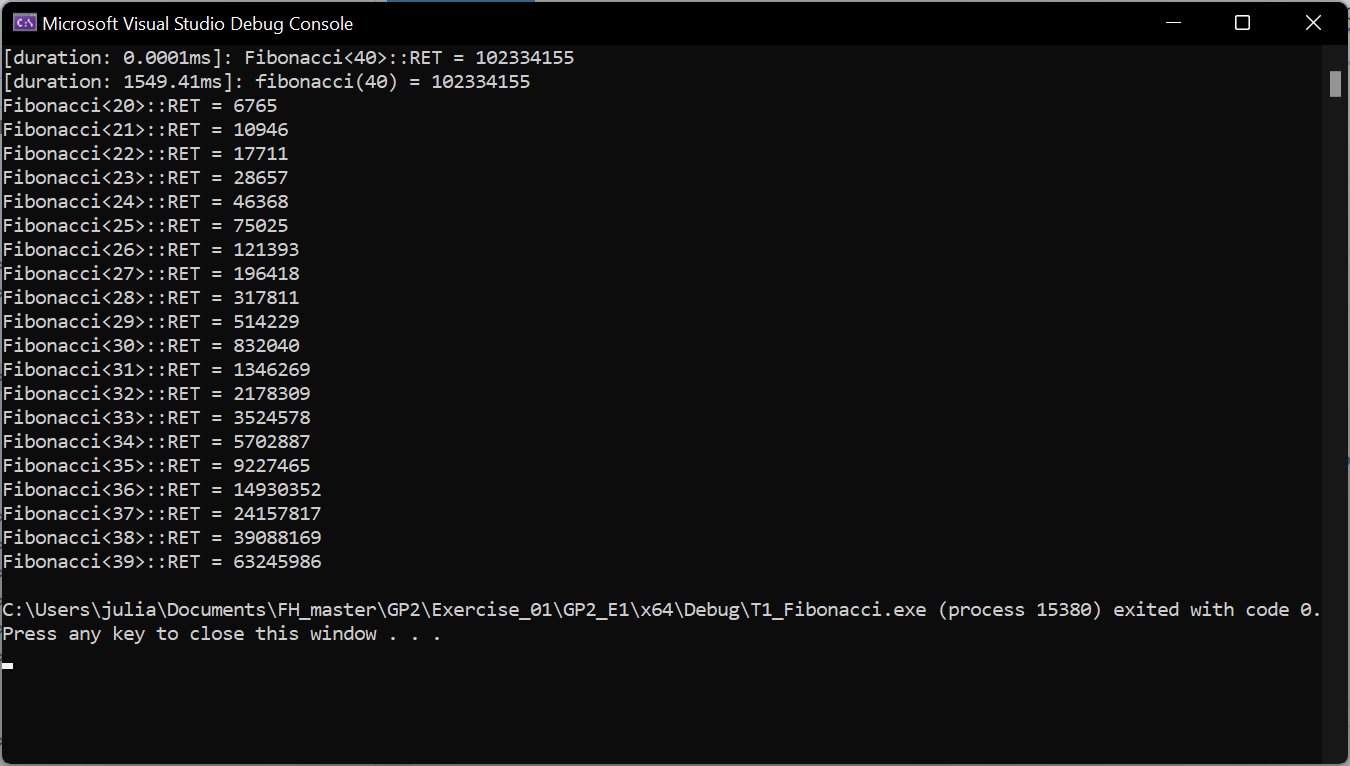
\includegraphics[width=.95\textwidth]{01_fib_test}
\caption{Testausgabe: Fibonacci}
\label{fig:01_fib_test}
\end{figure}

\clearpage

%%%-----------------------------------------------------------------------------

\section{1, 2, 3, 4, 5, 6, 7, \dots}

\subsection{Lösungsidee}

Ein Counter hat zwei dynamisch gebundene Methoden, welche von ableitenden Klassen 
überschrieben werden können. Die Methode \texttt{protected T get\_step\_size()} 
liefert die Schrittgröße des Counters. Die Methode \texttt{public void increment()} 
inkrementiert den aktuellen Counter-Value um die Schrittgröße. 
Der \texttt{BoundedCounter} überschreibt \texttt{increment()} und verhindert, 
dass der \texttt{bound} überschritten wird. Dies wird erreicht indem die 
Implementierung der Basisklasse aufgerufen wird und der Counter-Value im Falle 
einer Überscheitung des bounds auf den vorherigen Wert zurückgesetzt wird.
Der \texttt{VarIncrement\-Counter} überschreibt \texttt{get\_step\_size()} und 
ändert so die Schrittgröße des Counters.

\subsection{Code}

\lstinputlisting[caption=Counter.h, language={[11]C++}]{src/Counters/Counter.h}
\lstinputlisting[caption=BoundedCounter.h, language={[11]C++}]{src/Counters/BoundedCounter.h}
\lstinputlisting[caption=VarIncrementCounter.h, language={[11]C++}]{src/Counters/VarIncrementCounter.h}
\lstinputlisting[caption=Configurations.h, language={[11]C++}]{src/Counters/Configurations.h}
\lstinputlisting[caption=CounterTests.h, language={[11]C++}]{src/Counters/CounterTests.h}
\lstinputlisting[caption=CounterTests.cpp, language={[11]C++}]{src/Counters/CounterTests.cpp}
\lstinputlisting[caption=main.cpp, language={[11]C++}]{src/Counters/main.cpp}

\subsection{Test}

\begin{figure}
\centering
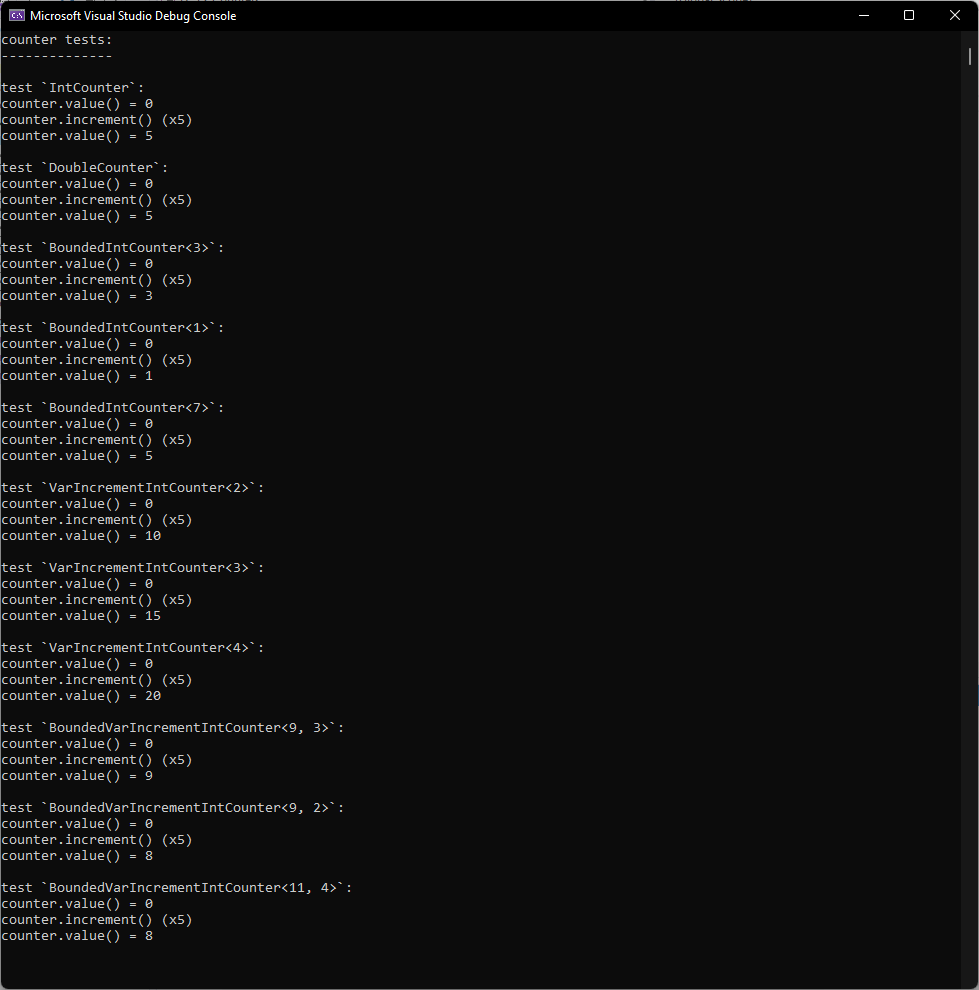
\includegraphics[width=.95\textwidth]{02_counter_test}
\caption{Testausgabe: Counter Test}
\label{fig:02_counter_test}
\end{figure}

\clearpage

%%%-----------------------------------------------------------------------------

\section{Counters off the Shelf}

\subsection{Lösungsidee}

\subsubsection{Template-Parameter des Generators}

\lstinputlisting[caption=CounterGenerator.h, language={[11]C++}, firstnumber=22, firstline=22, lastline=26]{src/Counters/CounterGenerator.h}

Alle Template-Parameter, bis auf den Datentyp des Zählers, haben einen Default-Wert.

\subsubsection{Optional}

Das \texttt{struct} \texttt{Optional} bzw. die Sub-structs \texttt{Empty} 
und \texttt{Value} haben eine Konstante \texttt{has\_value}, 
mit der gerüft werden kann, ob der übergebene Parameter einen 
gültigen Wert enthält bzw. ob der übergebene Parameter bei der 
Generierung der Konfiguration berücksichtigt werden soll. 
Dies ist für diesen Anwendungsfall sinnvoll, weil so \zB 
für den letzten Template-Parameter explizit ein "Wert" übergeben 
werden kann, während für den vorletzten Parameter der Default-Wert 
erhalten werden kann indem \texttt{Empty} übergeben wird.

\subsubsection{Hierarchie}

Die Verschachtelung \bzw die Ableitungshierarchie wird mittels der 
TMF \texttt{IF} aufgebaut.

\subsection{Code}

\lstinputlisting[caption=TMFs.h, language={[11]C++}]{src/Counters/TMFs.h}
\lstinputlisting[caption=CounterGenerator.h, language={[11]C++}]{src/Counters/CounterGenerator.h}
\lstinputlisting[caption=GeneratorTests.h, language={[11]C++}]{src/Counters/GeneratorTests.h}
\lstinputlisting[caption=GeneratorTests.cpp, language={[11]C++}]{src/Counters/GeneratorTests.cpp}

\subsection{Test}

\begin{figure}[h]
\centering
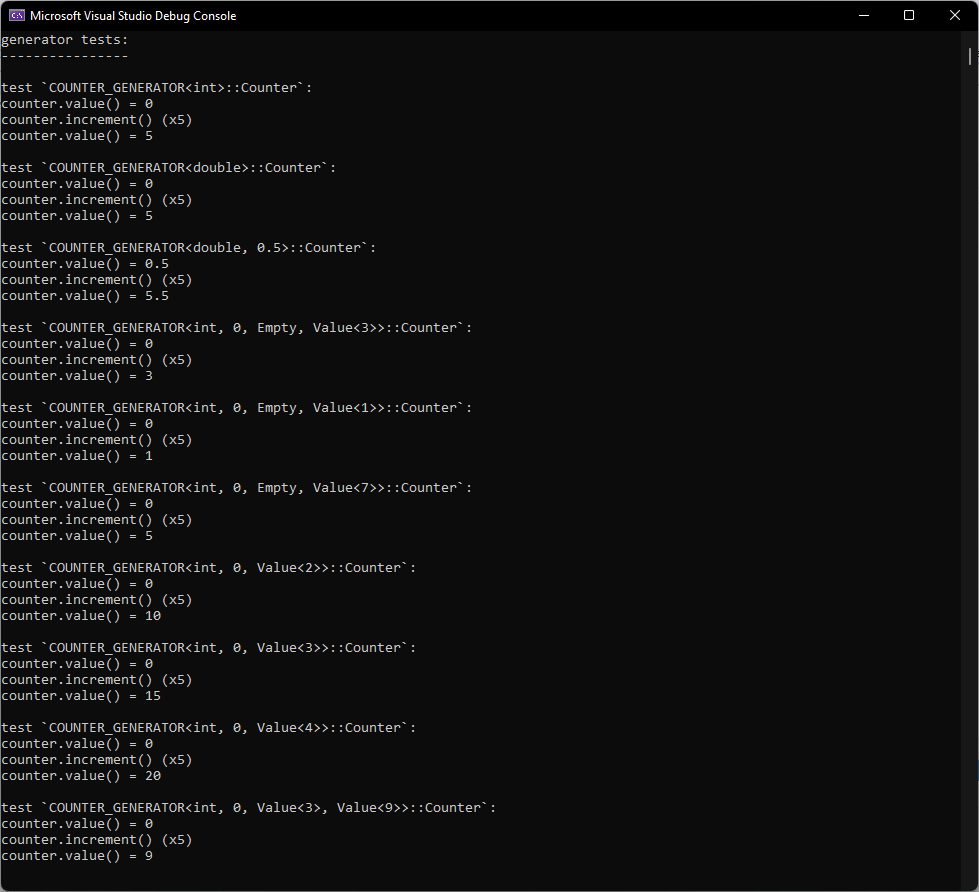
\includegraphics[width=.95\textwidth]{03_generator_test}
\caption{Testausgabe: Generator Test (Teil 1)}
\label{fig:03_generator_test}
\end{figure}

\begin{figure}[h]
\centering
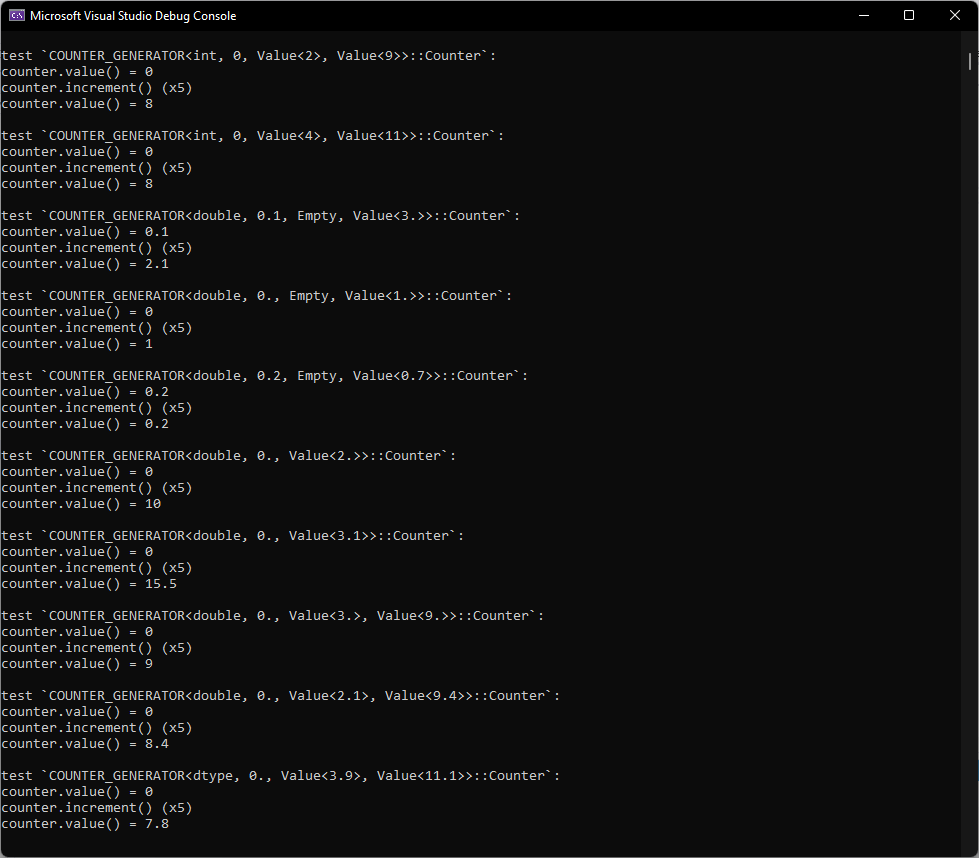
\includegraphics[width=.95\textwidth]{04_generator_test}
\caption{Testausgabe: Generator Test (Teil 2)}
\label{fig:04_generator_test}
\end{figure}

%%%-----------------------------------------------------------------------------

% \section*{Zusammenfassung und Anmerkungen}

%%%-----------------------------------------------------------------------------

% \section*{Quellen}

% \printbibliography[heading=noheader]

%%%-----------------------------------------------------------------------------
\end{document}
%%%-----------------------------------------------------------------------------